\begin{lpu}

Nachdem Sie bereits zwei Arten von Algorithmen kennengelernt haben — einen für die Klassifikation und die lineare Regression — begegnet Ihnen nun eine dritte: die \textbf{Ballung}, auch \emph{clustering} genannt. Während bei der Entwicklung für Algorithmen der Klassifikation und Regression jeweils die \emph{richtige Antwort} vorgegeben ist (man spricht von \emph{überwachtem Lernen}), ist dies bei Ballung nicht der Fall: Sie erkennen Strukturen in Daten, ohne dass jemand vorher gesagt hat, wie viele Gruppen es gibt oder wie diese aussehen sollen.

Ein typisches Beispiel: Ein Onlineshop möchte seine Kundschaft segmentieren, um gezieltere Werbung zu machen. Dazu werden Merkmale wie Bestellverhalten oder Preisempfindlichkeit betrachtet – ohne zu wissen, wie viele «Typen» von Kundinnen und Kunden es gibt. Stellen Sie sich also vor, Sie betrieben einen Online-Shop für Elektronik. In Ihrem System liegen Daten vor über alle Bestellungen der letzten zwei Jahre: Wie teuer war die Bestellung? Zu welcher Tageszeit wurde sie getätigt? Welche Produktkategorien waren beteiligt? Nun möchten Sie Ihre Kundschaft \textit{segmentieren} (also in Gruppen einteilen), um gezieltere Angebote zu machen:

Sie möchten für diese Gruppen unterschiedliche Rabatte oder Newsletter formulieren – wissen aber nicht im Voraus, wie viele Gruppen existieren oder wie diese genau definiert sind. Hier kommt ein Ballungsalgorithmus ins Spiel: Er gruppiert die vorhandenen Daten in sinnvolle \textit{cluster} (= Gruppen), basierend auf Ähnlichkeiten zwischen ihnen.

Ein anderes Beispiel: Stellen Sie sich vor, Spotify möchte auswerten, wie sich verschiedene Nutzerinnen und Nutzer verhalten. Jede Person hört unterschiedlich oft Musik, zu verschiedenen Tageszeiten, in verschiedenen Genres. Spotify kann diese Daten verwenden, um Nutzerinnen und Nutzer automatisch in Gruppen einzuteilen und für diese Gruppen geeignete Vorschläge zu machen. Beispielsweise könnte ein \textit{clustering}-Algorithmus automatisch herausfinden, dass es folgende Gruppen gibt:

\begin{itemize}
  \item Lernende, die tagsüber ruhige Musik hören.
  \item Sportlich Aktive, die vorwiegend Beats am Abend hören.
  \item Gelegenheitshörerinnen, die ab und zu einen Hit-Remix streamen.
\end{itemize}

Wichtig zu verstehen ist, dass hier niemand \textit{a priori} sagt, dass es diese Kategorien gibt, sondern sich diese aus den Daten direkt ergeben. 

\begin{theorie}
Dies nennt man \textbf{unüberwachten Lernen} (\emph{unsupervised learning}). Hier versucht ein Algorithmus, Strukturen oder Muster in einem Datensatz zu erkennen, \textbf{ohne dass richtige Antworten vorgegeben sind}. Es gibt also keine Labels, keine Zielwerte. Stattdessen werden Ähnlichkeiten in den Daten genutzt, um Gruppen (\textit{cluster}), Ausreisser oder Ordnungen zu finden. Diese Algorithmen sind nützlich, wenn Sie in Daten verborgene Strukturen aufdecken wollen, ohne vorab zu wissen, welche Kategorien es gibt.
\end{theorie} 


\begin{aufgabe}{1}
Lesen Sie den folgenden Absatz und beantworten Sie anschliessend die Fragen:

\emph{Stellen Sie sich nun vor, Sie betrieben einen solchen Onlinehandel, wie oben beschrieben, selber. In Ihrem Kundenstamm gibt es verschiedene Typen: Einige kaufen spontan und achten stark auf Preisaktionen. Andere planen ihren Einkauf langfristig, aber kaufen bevorzugt Premiumprodukte. Vermutlich gibt es aber auch noch viele andere Typen! Wenn Sie Kunden der jeweiligen Typen unterschiedliche Angebote machen könnten – wie würden Sie herausfinden, wie viele Gruppen es gibt, und wer zu welcher gehört?}

\begin{itemize}
  \item Warum sind in dieser Situation keine Kategorien im Voraus bekannt?
  \item Warum kann ein Entscheidungsbaum hier nicht angewendet werden?
  \item Welche Vorteile könnte es haben, solche Gruppen automatisch zu erkennen?
\end{itemize}
\end{aufgabe}

Wir wechseln nun das Beispiel zum letzten Mal, und nehmen zur Hand das Parade-Beispiel für die Ballung: Sie besitzen eine Kette von Pizza-Kurieren, welche in einer grossen Stadt mehrere Standorte haben. Nachfolgend finden Sie eine Grafik, wo die meisten Bestellungen getätigt werden. 

\begin{figure}[h]
\centering
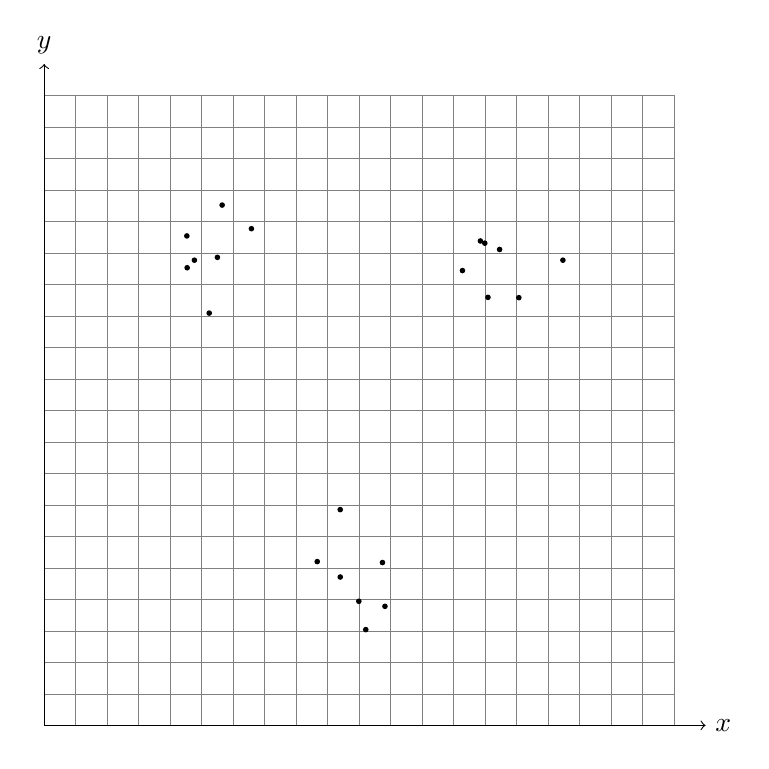
\begin{tikzpicture}[scale=0.4]
\draw[step=1cm,gray,very thin] (0,0) grid (20,20);
\draw[->] (0,0) -- (21,0) node[right] {$x$};
\draw[->] (0,0) -- (0,21) node[above] {$y$};

\filldraw[black] (5.50,14.86) circle (2pt);
\filldraw[black] (5.65,16.52) circle (2pt);
\filldraw[black] (4.77,14.77) circle (2pt);
\filldraw[black] (6.58,15.77) circle (2pt);
\filldraw[black] (4.53,15.54) circle (2pt);
\filldraw[black] (4.54,14.53) circle (2pt);
\filldraw[black] (5.24,13.09) circle (2pt);

\filldraw[black] (13.28,14.44) circle (2pt);
\filldraw[black] (13.99,15.31) circle (2pt);
\filldraw[black] (14.09,13.59) circle (2pt);
\filldraw[black] (16.47,14.77) circle (2pt);
\filldraw[black] (15.07,13.58) circle (2pt);
\filldraw[black] (14.46,15.11) circle (2pt);
\filldraw[black] (13.85,15.38) circle (2pt);

\filldraw[black] (9.40,4.71) circle (2pt);
\filldraw[black] (9.40,6.85) circle (2pt);
\filldraw[black] (9.99,3.94) circle (2pt);
\filldraw[black] (10.82,3.78) circle (2pt);
\filldraw[black] (10.21,3.04) circle (2pt);
\filldraw[black] (8.67,5.20) circle (2pt);
\filldraw[black] (10.74,5.17) circle (2pt);

% Aufgabe: Tragen Sie hier Ihre drei Depot-Standorte ein, z.B.:
% \filldraw[red] (x,y) node[below right]{Depot 1} circle (4pt);

\end{tikzpicture}
\caption{Bestellungen als Punkte im Stadtgebiet}
\label{fig:pizza_kmeans_example}
\end{figure}

Da Sie wissen, dass das Geheimnis des Erfolges Ihres Unternehmens darin liegt, dass die Pizza so nah wie möglich an Ihren Kunden produziert wird (um schnelle Lieferzeiten und eine höhere Knusprigkeit des Pizzarandes zu gewährleisten), möchten Sie neue Standorte aufbauen, die möglichst nah an möglichst vielen Kunden liegen. Im Beispiel oben ist das nicht schwierig, aber wie sieht es im nachfolgenden Beispiel aus?

\begin{figure}[h]
\centering
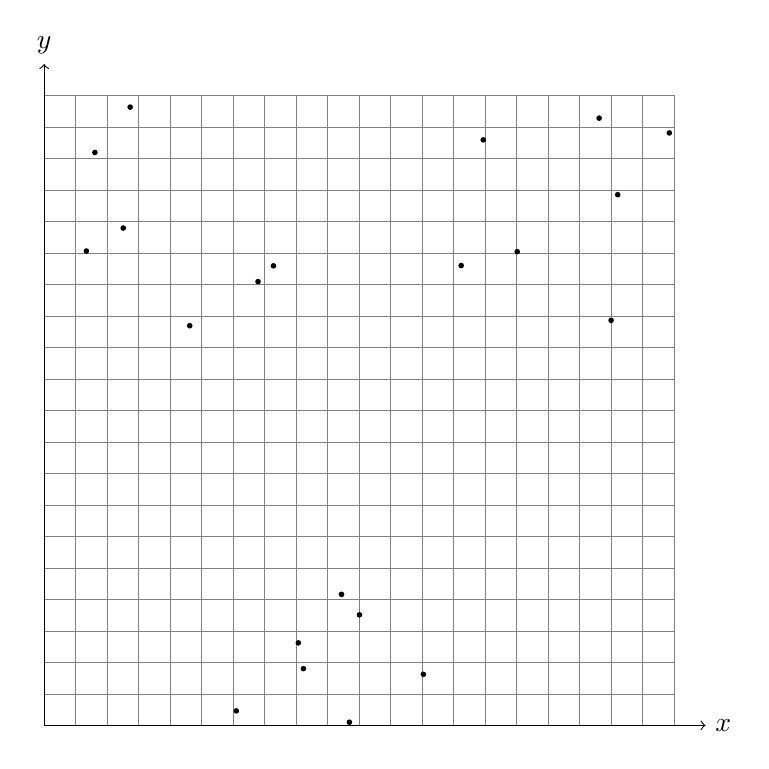
\begin{tikzpicture}[scale=0.4]
\draw[step=1cm,gray,very thin] (0,0) grid (20,20);
\draw[->] (0,0) -- (21,0) node[right] {$x$};
\draw[->] (0,0) -- (0,21) node[above] {$y$};

\filldraw[black] (1.61,18.19) circle (2pt);
\filldraw[black] (4.62,12.69) circle (2pt);
\filldraw[black] (2.73,19.63) circle (2pt);
\filldraw[black] (1.34,15.06) circle (2pt);
\filldraw[black] (6.79,14.09) circle (2pt);
\filldraw[black] (2.51,15.79) circle (2pt);
\filldraw[black] (7.28,14.59) circle (2pt);

\filldraw[black] (15.02,15.04) circle (2pt);
\filldraw[black] (19.85,18.81) circle (2pt);
\filldraw[black] (18.21,16.85) circle (2pt);
\filldraw[black] (17.62,19.28) circle (2pt);
\filldraw[black] (13.94,18.59) circle (2pt);
\filldraw[black] (13.24,14.60) circle (2pt);
\filldraw[black] (18.00,12.86) circle (2pt);

\filldraw[black] (9.69,0.10) circle (2pt);
\filldraw[black] (9.44,4.16) circle (2pt);
\filldraw[black] (6.10,0.46) circle (2pt);
\filldraw[black] (12.04,1.62) circle (2pt);
\filldraw[black] (10.01,3.51) circle (2pt);
\filldraw[black] (8.07,2.62) circle (2pt);
\filldraw[black] (8.23,1.80) circle (2pt);

% Aufgabe: Tragen Sie hier Ihre drei Depot-Standorte ein, z.B.:
% \filldraw[red] (x,y) node[below right]{Depot 1} circle (4pt);

\end{tikzpicture}
\caption{Verstreut liegende Pizzabestellungen}
\label{fig:pizza_kmeans_variante}
\end{figure}

\begin{aufgabe}{2}
In Abbildung~\ref{fig:pizza_kmeans_variante} sehen Sie also die Positionen von Pizzabestellungen in einer Stadt. Die Punkte sind diesmal deutlich unregelmässiger verteilt als im vorherigen Beispiel. Sie möchten drei neue Depots eröffnen, von denen die Pizzas geliefert werden. Ziel ist es, dass:

\begin{itemize}
  \item jede Bestellung möglichst nah bei einem Depot liegt,
  \item die Depots möglichst gleichmässig ausgelastet sind.
\end{itemize}

\vspace{1em}
\textbf{1. Gruppieren Sie von Hand}

\begin{itemize}
  \item Versuchen Sie, die Punkte visuell in drei Gruppen zu unterteilen.
  \item Zeichnen Sie mit Farbstiften oder Markierungen ein, welche Punkte Sie jeweils zusammenfassen würden.
  \item Überlegen Sie: Was macht eine ``gute'' Gruppe aus?
\end{itemize}

\vspace{1em}
\textbf{2. Wählen Sie Gruppenzentren}

\begin{itemize}
  \item Bestimmen Sie für jede Gruppe ein Zentrum (einen ``günstigen'' Ort für ein Depot).
  \item Notieren Sie sich die Koordinaten der Zentren.
  \item Warum haben Sie genau diese Punkte gewählt?
\end{itemize}

\vspace{1em}
\textbf{3. Denken Sie einen Schritt weiter}

\begin{itemize}
  \item Wenn Sie nun nur die Zentren betrachten: Könnte man jedem Punkt \emph{automatisch} das nächstgelegene Zentrum zuweisen, ungeachtet dessen, welcher (Start-)Gruppe dieser Punkt zugewiesen war?
  \item Und wenn Sie dadurch neue Gruppen erhalten – wie könnten Sie dann neue Zentren berechnen?
  \item Wiederholen Sie diesen Schritt (Zuweisen $\rightarrow$ Zentren berechnen) gedanklich ein weiteres Mal.
\end{itemize}

\vspace{1em}
\textbf{4. Reflektieren Sie:}

\begin{itemize}
  \item Was würde passieren, wenn Sie diesen Prozess so lange wiederholen, bis sich nichts mehr verändert?
  \item Haben Sie dabei etwas entdeckt, was vielleicht auch ein Computer tun könnte?
\end{itemize}
\end{aufgabe}

Sie haben gerade selbst die Grundidee des \textbf{\textit{k-means}-Algorithmus} entdeckt – ein Verfahren, das Gruppen findet, indem es immer wieder Gruppenzugehörigkeiten aktualisiert und neue Gruppenzentren berechnet. Während Sie sich hier noch auf Ihre Intuition verlassen haben, um die ersten Gruppierungen und Zentren zu bestimmen, verfügt ein Computer nicht über eine Intuition. An deren Stelle rückt der Zufall:

\begin{theorie}
Ein verbreiteter Algorithmus zur Ballung ist \textbf{\textit{k-means}}. Er teilt Datenpunkte in genau $k$ Gruppen (Ballungen), sodass jeder Punkt zu dem Zentrum gehört, zu dem er die kleinste Distanz hat.

Die Schritte des Algorithmus:
\begin{enumerate}
  \item Wähle $k$ zufällige Punkte als Start-Zentren.
  \item Ordne jeden Datenpunkt dem nächsten Zentrum zu ($\Rightarrow$ erste Ballungen).
  \item Berechne für jede Ballung den Mittelpunkt (\textit{Zentroid}).
  \item Wiederhole Schritt 2–3, bis sich die Zentren nicht mehr (viel) verändern.
\end{enumerate}

Die Distanz zwischen Datenpunkten $x$ und $c$ wird dabei durch die \textbf{euklidische Distanz} gemessen:
\[
\text{dist}(p, c) = \sqrt{(p^{(x)} - c^{(x)})^2 + (p^{(y)} - c^{(y)})^2}
\]

Allgemein (für $d$ Dimensionen):
\[
\text{dist}(p, c) = \sqrt{ \sum_{i=1}^d (p^{(i)} - c^{(i)})^2 }
\]

Sobald alle Punkte einer Gruppe zugewiesen sind, wird für jede Gruppe $G_j$ ein neues Gruppenzentrum (Zentroid) $c_j$ (wie \textit{centroid}) berechnet – als \textbf{Mittelwert} aller Punkte in dieser Gruppe.

\vspace{0.5em}
\textbf{Berechnung des Gruppenzentrums (Zentroid)}

Für jede Gruppe \( G_j \) mit Punkten \( x_1, x_2, \dots, x_n\) berechnet man das neue Zentrum \( c_j\) indem jede Koordinate separat gemittelt wird:

\[
c_j^{(k)} = \frac{1}{|G_j|} \sum_{x_i \in G_j} x_i^{(k)} \quad \text{für } k = 1, 2, \dots, d
\]

Der vollständige Zentroid ergibt sich also als:
\[
c_j = \left( \frac{1}{|G_j|} \sum_{x_i \in G_j} x_i^{(1)},\ 
             \frac{1}{|G_j|} \sum_{x_i \in G_j} x_i^{(2)},\ 
             \dots,\ 
             \frac{1}{|G_j|} \sum_{x_i \in G_j} x_i^{(d)} \right)
\]

Das heisst: Jede Koordinate des Zentroids ist der Mittelwert der entsprechenden Koordinaten aller Punkte der Gruppe.
\end{theorie}

Auch wenn das mathematisch involviert scheinen mag, so ist der Algorithmus einfach zu verstehen. Folgende Simulation kann Ihnen helfen, sich das vorgehen des \textit{k-means} zu verbildichen:

\begin{aufgabe}{3}
Benutzen Sie \href{https://www.naftaliharris.com/blog/visualizing-k-means-clustering/}{diese Simulation}\footnote{\href{https://www.naftaliharris.com/blog/visualizing-k-means-clustering/}{\url{naftaliharris.com/blog/visualizing-k-means-clustering/}}}, um sich ein Bild davon zu machen, wie \textit{k-means} funktioniert. Beginnen Sie dort mit \tikz[baseline=(X.base)]
  \node[draw=black, rounded corners, inner xsep=2pt, inner ysep=1pt]
  (X) {\textsf{Randomly}}; für \textit{How to pick the initial centroids?}; dann wählen Sie zunächst \tikz[baseline=(X.base)]
  \node[draw=black, rounded corners, inner xsep=2pt, inner ysep=1pt]
  (X) {\textsf{Gaussian Mixture}};. Spielen Sie im Anschluss mit verschiedene Einstellungen!


\vspace{0.5em}
Beantworten Sie danach folgende Fragen:

\begin{itemize}
  \item Was passiert, wenn zwei Zentren sehr nahe beieinander liegen? (Dazu können Sie zu Beginn der Simulation \tikz[baseline=(X.base)]
  \node[draw=black, rounded corners, inner xsep=2pt, inner ysep=1pt]
  (X) {\textsf{I'll Choose}}; wählen.)
  \item Wie verhält sich der Algorithmus bei ``nicht-runden'' Gruppenformen?
  \item Ist die Wahl der Startpunkte wichtig?
\end{itemize}
\end{aufgabe}

Obwohl Sie für gewöhnlich sich diese Berechnungen von einem Computer ausführen lassen (wie wir später auch sehen werden), ist es lehrreich, wenn Sie einmal zumindest die Berechnung mit Ihrem eigenen Gehirn ausführen.


\begin{aufgabe}{4*}
In dieser Aufgabe wenden Sie den \textit{k-means}-Algorithmus auf ein ganz kleines Beispiel in zwei Dimensionen an. Die Punkte sind:

\[
A = (2, 2),\quad B = (3, 4),\quad C = (5, 3),\quad D = (8, 7)
\]

\begin{center}
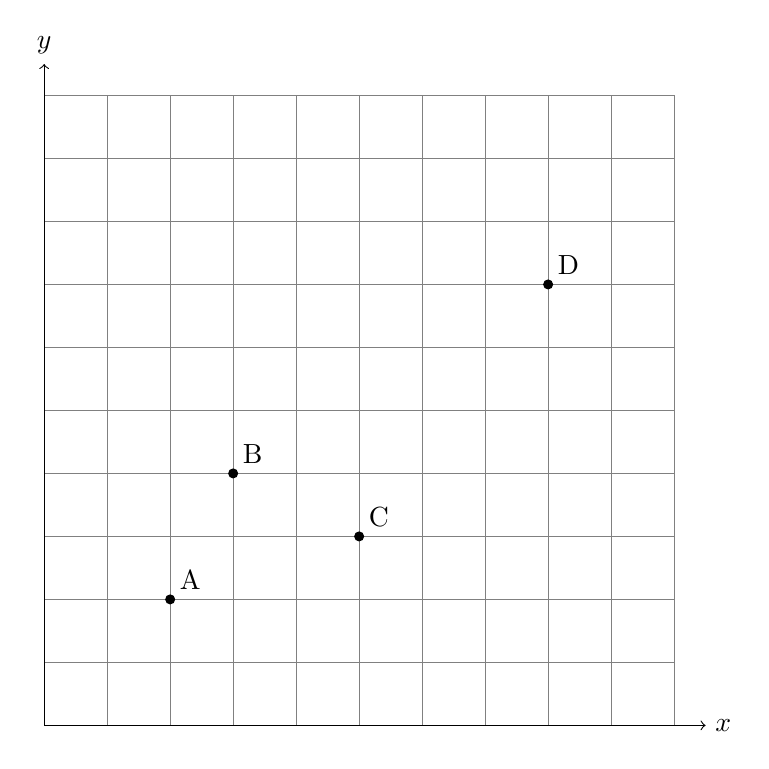
\begin{tikzpicture}[scale=0.8]
  \draw[step=1cm,gray,very thin] (0,0) grid (10,10);
  \draw[->] (0,0) -- (10.5,0) node[right] {$x$};
  \draw[->] (0,0) -- (0,10.5) node[above] {$y$};

  % Datenpunkte
  \filldraw[black] (2,2) circle (2pt) node[above right] {A};
  \filldraw[black] (3,4) circle (2pt) node[above right] {B};
  \filldraw[black] (5,3) circle (2pt) node[above right] {C};
  \filldraw[black] (8,7) circle (2pt) node[above right] {D};

  % Startzentren
  % \draw[red, thick] (2,2) node[below left] {\textcolor{red}{$Z_1^{(0)}$}} node[cross, red, thick, minimum size=8pt] {};
  % \draw[red, thick] (8,7) node[below right] {\textcolor{red}{$Z_2^{(0)}$}} node[cross, red, thick, minimum size=8pt] {};

\end{tikzpicture}
\end{center}

Wir möchten die Punkte in $k = 2$ Gruppen einteilen.

\begin{enumerate}
  \item \textbf{Start:} Wählen Sie zwei Startzentren ``zufällig''.

  \item \textbf{Zuweisungsschritt:} Berechnen Sie für jeden Punkt der 4 Punkte die euklidische Distanz zu beiden Zentren und ordnen Sie ihn dem nächstgelegenen Startzentrum zu.

  \item \textbf{Zentroid-Schritt:} Berechnen Sie für jede Gruppe den neuen Mittelpunkt (Zentroid) als arithmetischen Mittelwert der Punkte.

  \item \textbf{Wiederholen:} Führen Sie einen weiteren Zuweisungsschritt mit den neuen Zentren durch. Ändern sich die Gruppen? Falls nein: Der Algorithmus ist fertig! Falls ja: Fangen Sie bei Schritt 2. wieder an, und beobachten Sie, wie sich die Zentroide und Gruppen verändern.

\end{enumerate}
\end{aufgabe}
\end{lpu}

\subsection*{Didaktische Überlegungen}


Das Thema ``Ballung'' (\textit{clustering}) stellt eine neue Denkweise im maschinellen Lernen dar: Erstmals arbeiten die SuS mit einem \emph{unüberwachten Verfahren}, bei dem die ``richtigen Antworten'' nicht vorgegeben sind. Statt zwischen Kategorien zu unterscheiden (Klassifikation) oder Werte vorherzusagen (Regression), geht es hier darum, in rohen Daten Muster zu entdecken, ohne dass diese explizit benannt sind. Diese Art des maschinellen Lernens wurde hier bewusst so früh wie möglich eingeführt, damit die SuS ein Konzept vom ML formen, das sowohl überwachtes als auch unüberwachtes Lernen einschliesst, und nicht einen Konzeptwandel vollbringen müssen.

Die vorgeschalteten Aufgaben, in denen SuS Standorte für einen Pizzalieferdienst setzen sollen, bevor der Algorithmus \textit{k-means} überhaupt eingeführt wird, dienen dazu, ein intuitives Verständnis für \textit{cluster} zu entwickeln. Sie lernen, dass Daten sinnvoll gruppiert werden können, auch wenn keine Etikette existiert.

Durch die strukturierte Heranführung an \textit{k-means} – erst durch Ausprobieren, dann durch Theorie, dann durch Visualisieren und zuletzt durch eigenes Berechnen — wird der Algorithmus ``sanft'' eingeführt. Die Verwendung konkreter Koordinaten in der letzten Aufgabe (``\textit{k-means} von Hand durchrechnen'') erlaubt es, das Verfahren schrittweise nachzuvollziehen. Diese Aufgabe ist nicht zwingend erforderlich für alle SuS, kann aber für leistungsstärkere Gruppen eine wertvolle Gelegenheit darstellen, sich mit dem mathematischen Kern des Algorithmus auseinanderzusetzen.

Für schwächere SuS kann diese letzte Aufgabe weggelassen werden, ohne dass das Grundverständnis für \textit{clustering} verloren geht. Alternativ kann sie als Partner- oder Gruppenarbeit gelöst werden.

\subsubsection*{Mathematische Vertiefung: Vergleich MSE und euklidischer Distanz}

Didaktisch lohnend könnte auch der Vergleich der euklidischen Distanz (im Zuweisungsschritt von \textit{k-means}) mit dem MSE aus dem Kapitel~\ref{sec:regression} sein, der im Zusammenhang  mit der Regression eingeführt wurde. Trotz formaler Ähnlichkeit (beide minimieren summierte quadratische Abstände) verfolgen die beiden Verfahren konzeptionell unterschiedliche Ziele:

\begin{itemize}
  \item Beim MSE werden Fehlerquadrate über \textbf{eine feste Referenz} (z.\,B.\ eine Gerade) berechnet, und der Mittelwert dieser Abweichungen dient der Optimierung.
  \item Beim \textit{clustering} hingegen dient die euklidische Distanz dazu, Punkte \textbf{dynamisch} einem Zentrum zuzuordnen. Die Zentren verändern sich selbst in jedem Schritt.
\end{itemize}

Diese Unterscheidung ist besonders fruchtbar im Hinblick auf Kompetenzaufbau: SuS lernen, dass mathematische Werkzeuge (wie Abstandsmasse) je nach Kontext unterschiedliche Bedeutungen und Funktionen erhalten können.


\subsection*{Musterlösungen}

\begin{aufgabe}{1}
\begin{itemize}
  \item \textbf{Warum sind in dieser Situation keine Kategorien im Voraus bekannt?}

    In dieser Situation liegen keine vordefinierten Labels oder Klassen vor, wie zum Beispiel ``Typ A'' oder ``Typ B''. Es handelt sich um \textbf{Verhaltensmuster}, die sich aus vielen Einzelinformationen (z.\,B.\ Kaufhäufigkeit, Produkttyp, Zeitpunkt, Rabattnutzung) ergeben. Welche Kundentypen überhaupt existieren, ist unbekannt – sie müssen erst aus den Daten erschlossen werden.

    In der Fachsprache handelt es sich deshalb um ein \textbf{unüberwachtes Lernproblem} (\textit{unsupervised learning}), weil keine ``richtigen Antworten'' als Trainingsdaten gegeben sind.

  \item \textbf{Warum kann ein Entscheidungsbaum hier nicht angewendet werden?}

Entscheidungsbäume gehören zum \textbf{überwachten Lernen}. Sie benötigen für jeden Eintrag im Datensatz ein sogenanntes ``Label'' – also eine Zielkategorie, die vom Modell gelernt werden soll (z.\,B.\ ``Kundentyp A''). In unserem Fall liegen jedoch keine solchen vorgegebenen Gruppen vor: Wir wissen nicht, wie viele Typen es gibt, und wir haben keine Information darüber, welcher Kunde zu welcher Gruppe gehört. Deshalb ist ein Entscheidungsbaum hier nicht einsetzbar.

\textbf{Wichtig:} Das Problem liegt \emph{nicht} an der Art der Eingangsdaten. Sowohl Entscheidungsbäume als auch Ballungs-Verfahren wie \textit{k-means} können grundsätzlich mit numerischen und kategorischen Daten umgehen (z.\,B.\ ``bestellt häufig'', ``Zahlungsart = Kreditkarte'', ``durchschnittlicher Warenkorbwert''). Entscheidend ist allein, ob es ein bekanntes Zielattribut (Label) gibt. In unserem Fall fehlt dieses – und deshalb ist ein \textbf{unüberwachter Lernalgorithmus} erforderlich.


  \item \textbf{Welche Vorteile könnte es haben, solche Gruppen automatisch zu erkennen?}

    Die automatische Gruppierung der Kundinnen und Kunden bringt mehrere Vorteile:
    \begin{itemize}
  \item \textbf{Personalisierte Angebote:} Verschiedene Gruppen können gezielt mit passenden Aktionen oder Produktempfehlungen angesprochen werden (z.\,B.\ Rabattgutscheine für preisbewusste Käuferinnen und Käufer, exklusive Neuheiten für Premiumkundschaft).

  \item \textbf{Besseres Kundenverständnis:} Der Algorithmus kann Muster aufdecken, die für Menschen nicht unmittelbar erkennbar sind. Dadurch entsteht ein tieferes, datenbasiertes Verständnis für das Verhalten und die Interessen der Kundschaft.

  \item \textbf{Weniger menschlicher Bias:} Da keine Kategorien im Vorfeld festgelegt werden müssen, entsteht weniger Verzerrung durch Vorurteile oder Annahmen der Entwicklerinnen und Entwickler. Gruppen entstehen rein datenbasiert – sofern die Daten selbst möglichst neutral sind.

  \item \textbf{Neue Gruppen entdecken:} Es können Gruppen auftauchen, an die niemand gedacht hat (z.\,B.\ ``Gelegenheitseinkäufer mit hohem Durchschnittspreis''). Dies ermöglicht neue Marketingstrategien oder Produktauswahl.

  \item \textbf{Skalierbarkeit:} Ein manuelles Durchforsten grosser Kundendatenbanken ist kaum möglich. Clustering-Algorithmen lassen sich hingegen auf sehr grosse Datenmengen anwenden – auch kontinuierlich und automatisiert.

  \item \textbf{Keine Zieldefinition notwendig:} Da keine vordefinierten ``richtigen Antworten'' nötig sind, eignet sich Clustering besonders in Situationen, wo das Ziel erst aus den Daten erschlossen werden soll – wie bei Marktanalysen oder Explorationsprojekten.
\end{itemize}
\end{itemize}
\end{aufgabe}

Die Aufgabe zielt darauf ab, dass SuS sich intuitiv mit der Idee der Clusterung auseinandersetzen. Eine mögliche Herangehensweise:

\begin{aufgabe}{2}
\begin{itemize}
  \item Die SuS erkennen, dass sich auf der Karte Gruppen von Punkten bilden — z.\,B.\ links oben, rechts oben und unten Mitte.
  \item Sie setzen drei Standorte so, dass sie in der Mitte dieser Gruppen liegen.
  \item Typischerweise wählen sie Zentren nahe $(5,15)$, $(15,15)$ und $(10,5)$.
\end{itemize}

\textbf{Begründung:} Diese Punkte minimieren \textit{visuell} in der Regel die durchschnittliche Distanz zur jeweiligen Gruppe, (``sie liegen in der Mitte'') und ermöglichen eine sinnvolle Auslastung der Standorte. Hier kann man anknüpfen und fragen, wie man den die ``Mitte'' mathematisch finden würde.

\textbf{Didaktisch wichtig:} Es gibt nicht ``die eine richtige Lösung'', sondern verschiedene plausible Gruppierungen. Die Diskussion darüber ist ausdrücklich Teil des Lernziels.
\end{aufgabe}








\begin{aufgabe}{3}
\begin{itemize}
  \item \textbf{Was passiert, wenn zwei Zentren sehr nahe beieinander liegen?}

    Wenn zwei Startzentren nahe beieinander liegen, erhalten sie zunächst sehr ähnliche oder sogar dieselben Punkte zugewiesen. Dies führt dazu, dass sich eines der Zentren entweder:
    
    \begin{itemize}
      \item in dieselbe Region bewegt wie das andere Zentrum, oder
      \item im Extremfall ``verwaist'' bleibt (d.\,h.\ keine Punkte zugewiesen bekommt).
    \end{itemize}

    Dadurch wird die effektive Anzahl der verwendeten Cluster reduziert – obwohl man eigentlich $k$ Gruppen erwartet hat. Es kann also passieren, dass ein Cluster ``verschwendet'' wird.

    In der Visualisierung sieht man, dass sich die beiden Zentren um dieselben Punkte ``streiten'', aber am Ende nur eines übrig bleibt. Dieses Verhalten zeigt, dass \textbf{\textit{k-means} empfindlich gegenüber der Startpunktwahl ist}.

  \item \textbf{Wie verhält sich der Algorithmus bei ``nicht-runden'' Gruppenformen?}

    \textit{k-means} basiert auf euklidischer Distanz und teilt den Raum in konvexe Regionen (Polygone), die durch die Nähe zu einem Zentrum definiert sind. Das funktioniert gut bei rundlichen, gleichmässig verteilten Gruppen, aber schlecht bei:

    \begin{itemize}
      \item länglichen, gebogenen oder ringförmigen Gruppen,
      \item Gruppen mit Ausstülpungen, ``Armen'' oder unregelmässiger Dichte,
      \item Gruppen mit sehr unterschiedlichen Varianzen.
    \end{itemize}

    In solchen Fällen kann \textit{k-means} Punkte falsch gruppieren, obwohl sie strukturell besser in einer anderen Gruppe aufgehoben wären. In der Demo sieht man dies z.\,B.\ beim ``Smile-Face''-Datensatz oder bei langgezogenen Strukturen.

  \item \textbf{Ist die Wahl der Startpunkte wichtig?}

    Ja, die Startpunkte sind \textbf{entscheidend} für das Ergebnis von \textit{k-means}. Da der Algorithmus auf lokaler Optimierung basiert, kann er in einem ``lokalen Minimum'' enden, das nicht optimal ist. Verschiedene Startpunkte können zu unterschiedlichen Gruppierungen führen, selbst wenn die Daten dieselben sind.

    In der Visualisierung wird deutlich:
    \begin{itemize}
      \item Günstig gewählte Startpunkte führen zu sinnvoll gruppierten Zentren.
      \item Ungünstige Startpunkte führen zu asymmetrischen, schlecht aufgeteilten oder instabilen Gruppierungen.
    \end{itemize}

    In der Praxis wird daher \textit{k-means} meist mehrfach mit zufälligen Startpunkten ausgeführt (sogenanntes \texttt{k-means++} oder ``Mehrfachinitialisierung''), und die beste Lösung wird dann aus diesen ausgewählt.
\end{itemize}
\end{aufgabe}

\begin{aufgabe}{4*}
Wir beginnen mit einfachen, ``zufälligen'' Startzentren: \( Z_1^{(0)} = A = (2,2),\ Z_2^{(0)} = D = (8,7) \)

\vspace{0.5em}
\textbf{1. Zuweisungsschritt:}

Berechne Distanzen zu den Zentren:

\[
\begin{array}{l|c|c|l}
\text{Punkt} & \text{Distanz zu } Z_1^{(0)} & \text{Distanz zu } Z_2^{(0)} & \text{Zugewiesen an} \\
\hline
A & 0.00 & \sqrt{(6)^2 + (5)^2} = 7.81 & Z_1 \\
B & \sqrt{1^2 + 2^2} = 2.24 & \sqrt{5^2 + 3^2} = 5.83 & Z_1 \\
C & \sqrt{3^2 + 1^2} = 3.16 & \sqrt{3^2 + 4^2} = 5.00 & Z_1 \\
D & 7.81 & 0.00 & Z_2 \\
\end{array}
\]

\vspace{0.5em}
\textbf{2. Neue Zentren berechnen:}

Gruppe \( Z_1 \) enthält \( A, B, C \):  
\[
Z_1^{(1)} = \left( \frac{2 + 3 + 5}{3}, \frac{2 + 4 + 3}{3} \right) = (3.33,\ 3.00)
\]

Gruppe \( Z_2 \): nur \( D \Rightarrow Z_2^{(1)} = (8,7) \)

\vspace{0.5em}
\textbf{3. Neuer Zuweisungsschritt:}

\[
\begin{array}{l|c|c|l}
\text{Punkt} & \text{Distanz zu } Z_1^{(1)} & \text{Distanz zu } Z_2^{(1)} & \text{Zugewiesen an} \\
\hline
A & \sqrt{(1.33)^2 + (1)^2} \approx 1.67 & 7.81 & Z_1 \\
B & \sqrt{(0.33)^2 + (1)^2} \approx 1.05 & 5.83 & Z_1 \\
C & \sqrt{(1.67)^2 + (0)^2} \approx 1.67 & 5.00 & Z_1 \\
D & 5.85 & 0.00 & Z_2 \\
\end{array}
\]

→ Keine Änderung der Gruppenzuweisung $\Rightarrow$ Algorithmus stoppt.

\vspace{0.5em}
\textbf{Endergebnis:}

\begin{itemize}
  \item Cluster 1: $A, B, C$ mit Zentrum bei $(3.33,\ 3.00)$
  \item Cluster 2: $D$ mit Zentrum bei $(8,\ 7)$
\end{itemize}
\end{aufgabe}


